% answers.tex —— 2006 年·普通高等学校招生考试·浙江卷理科 · 参考答案与详细解析片段
% 由 tools/generate_projects.py 依来源总账自 2006/2006_数学真题_浙江理_试题.md + 2006/2006_数学真题_浙江理_解析正文.md + 2006/2006_数学真题_浙江理_答案要点.md 生成，勿手改（改源 MD 后重跑）


\begin{gktip}
以下为依据固定候选题面独立求解的草稿，不是官方答案或解析。未使用未核验的答案材料。题面来源身份未认证。Q14 按通常的正投影约定；Q15 的 $M,N$ 按源图取最高点两侧相邻零点。
\end{gktip}

\begin{answer}
\gksolhead{1}{}

\textbf{题目}：

设集合 $A=\{x\mid -1\leqslant x\leqslant2\}$，$B=\{x\mid 0\leqslant x\leqslant4\}$，则 $A\cap B=$\mbox{（　　）}

\begin{gkopts}(4)
\task （A）$[0,2]$
\task （B）$[1,2]$
\task （C）$[0,4]$
\task （D）$[1,4]$
\end{gkopts}

\Needspace{4\baselineskip}
\textbf{解析}

$A\cap B=[0,2]$，选 A。

\gkanswer{答案：A。}

\end{answer}
\begin{answer}
\gksolhead{2}{}

\textbf{题目}：

已知 $\dfrac{m}{1+i}=1-ni$，其中 $m,n$ 是实数，$i$ 是虚数单位，则 $m+ni=$\mbox{（　　）}

\begin{gkopts}(4)
\task （A）$1+2i$
\task （B）$1-2i$
\task （C）$2+i$
\task （D）$2-i$
\end{gkopts}

\Needspace{4\baselineskip}
\textbf{解析}

$m/(1+i)=m(1-i)/2=1-ni$。比较实、虚部得 $m=2,n=1$，故 $m+ni=2+i$，选 C。

\gkanswer{答案：C（$2+i$）。}

\end{answer}
\begin{answer}
\gksolhead{3}{}

\textbf{题目}：

已知 $0<a<1$，$\log_a m<\log_a n<0$，则\mbox{（　　）}

\begin{gkopts}(4)
\task （A）$1<n<m$
\task （B）$1<m<n$
\task （C）$m<n<1$
\task （D）$n<m<1$
\end{gkopts}

\Needspace{4\baselineskip}
\textbf{解析}

$\log_a x$ 在 $0<a<1$ 时递减。由 $\log_a m<\log_a n$ 得 $m>n$；由 $\log_a n<0$ 得 $n>1$，故 $1<n<m$，选 A。

\gkanswer{答案：A。}

\end{answer}
\begin{answer}
\gksolhead{4}{}

\textbf{题目}：

\Needspace{5\baselineskip}
在平面直角坐标系中，不等式组
\nopagebreak[4]
\[
\begin{cases}
x+y-2\geqslant0,\\
x-y+2\geqslant0,\\
x\leqslant2
\end{cases}
\]
表示的平面区域的面积是\mbox{（　　）}

\begin{gkopts}(4)
\task （A）$4\sqrt2$
\task （B）$4$
\task （C）$2\sqrt2$
\task （D）$2$
\end{gkopts}

\Needspace{4\baselineskip}
\textbf{解析}

约束为 $y\ge2-x$、$y\le x+2$、$x\le2$。可行域顶点为 $(0,2),(2,0),(2,4)$，面积为 $4$，选 B。

\gkanswer{答案：B（4）。}

\end{answer}
\begin{answer}
\gksolhead{5}{}

\textbf{题目}：

若双曲线 $\dfrac{x^2}{m}-y^2=1$ 上的点到左准线的距离是到左焦点距离的 $\dfrac13$，则 $m=$\mbox{（　　）}

\begin{gkopts}(4)
\task （A）$\dfrac12$
\task （B）$\dfrac32$
\task （C）$\dfrac18$
\task （D）$\dfrac98$
\end{gkopts}

\Needspace{4\baselineskip}
\textbf{解析}

双曲线的 $a^2=m,b^2=1,c^2=m+1$。点到焦点的距离与到对应准线的距离之比为离心率 $e$，所以题给的反比为 $1/e=1/3$，即 $e=3$。于是 $(m+1)/m=9$，得 $m=1/8$，选 C。

\gkanswer{答案：C（$m=1/8$）。}

\end{answer}
\begin{answer}
\gksolhead{6}{}

\textbf{题目}：

函数 $y=\dfrac12\sin2x+\sin^2x$，$x\in\mathbb R$ 的值域是\mbox{（　　）}

（A）$\left[-\dfrac12,\dfrac32\right]$　（B）$\left[-\dfrac32,\dfrac12\right]$

（C）$\left[-\dfrac{\sqrt2}{2}+\dfrac12,\dfrac{\sqrt2}{2}+\dfrac12\right]$　（D）$\left[-\dfrac{\sqrt2}{2}-\dfrac12,\dfrac{\sqrt2}{2}-\dfrac12\right]$

\Needspace{4\baselineskip}
\textbf{解析}

\nopagebreak[4]
\[
y=\frac12+\frac12(\sin2x-\cos2x).
\]

括号内振幅为 $\sqrt2$，故值域为 $[\frac12-\frac{\sqrt2}{2},\frac12+\frac{\sqrt2}{2}]$，选 C。

\gkanswer{答案：C。}

\end{answer}
\begin{answer}
\gksolhead{7}{}

\textbf{题目}：

“$a>b>0$”是“$ab<\dfrac{a^2+b^2}{2}$”的\mbox{（　　）}

（A）充分而不必要条件　（B）必要而不充分条件

（C）充分必要条件　（D）既不充分也不必要条件

\Needspace{4\baselineskip}
\textbf{解析}

不等式等价于 $(a-b)^2>0$，即 $a\ne b$。$a>b>0$ 是其充分条件，但不必要，选 A。

\gkanswer{答案：A（充分而不必要条件）。}

\end{answer}
\begin{answer}
\gksolhead{8}{}

\textbf{题目}：

若多项式 $x^2+x^{10}=a_0+a_1(x+1)+\cdots+a_9(x+1)^9+a_{10}(x+1)^{10}$，则 $a_9=$\mbox{（　　）}

\begin{gkopts}(4)
\task （A）$9$
\task （B）$10$
\task （C）$-9$
\task （D）$-10$
\end{gkopts}

\Needspace{4\baselineskip}
\textbf{解析}

令 $u=x+1$，则 $x^2+x^{10}=(u-1)^2+(u-1)^{10}$。其中 $u^9$ 项系数为 $-\binom{10}{9}=-10$，选 D。

\gkanswer{答案：D（$-10$）。}

\end{answer}
\begin{answer}
\gksolhead{9}{}

\textbf{题目}：

如图，$O$ 是半径为 $1$ 的球心，点 $A,B,C$ 在球面上，$OA,OB,OC$ 两两垂直，$E,F$ 分别是大圆弧 $\widehat{AB}$ 与 $\widehat{AC}$ 的中点，则点 $E,F$ 在该球面上的球面距离是\mbox{（　　）}

\begin{gkopts}(2)
\task （A）$\dfrac{\pi}{4}$
\task （B）$\dfrac{\pi}{3}$
\task （C）$\dfrac{\pi}{2}$
\task （D）$\dfrac{\sqrt2\pi}{4}$
\end{gkopts}
\nopagebreak[4]
\begin{center}% Source: fixed 2006 Zhejiang science scan, PDF page 1, Q9.
% Schematic projection; retain the three mutually perpendicular radii and
% the arc-midpoint labels on the great-circle arcs AB and AC.
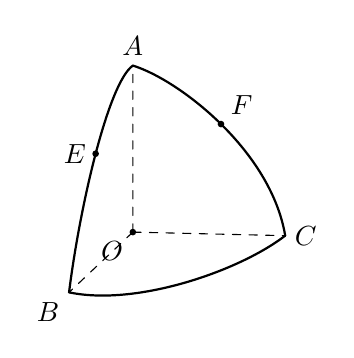
\begin{tikzpicture}[line cap=round,line join=round,x=0.9cm,y=0.9cm]
  \coordinate (O) at (0,0);
  \coordinate (A) at (0,2.35);
  \coordinate (B) at (-0.9,-0.85);
  \coordinate (C) at (2.15,-0.05);
  % Parameter midpoints of the two schematic cubic Bezier arcs.
  \coordinate (E) at (-0.525,1.10625);
  \coordinate (F) at (1.24375,1.525);
  % Schematic visible spherical boundary and the two great-circle arcs.
  \draw[thick] (A) .. controls (-0.35,2.1) and (-0.75,0.35) .. (B);
  \draw[thick] (A) .. controls (0.65,2.15) and (1.95,1.15) .. (C);
  \draw[thick] (B) .. controls (0.05,-1.05) and (1.5,-0.55) .. (C);
  \draw[dashed] (O)--(A) (O)--(B) (O)--(C);
  \fill (O) circle (1.2pt) (E) circle (1.2pt) (F) circle (1.2pt);
  \node[above] at (A) {$A$};
  \node[below left] at (B) {$B$};
  \node[right] at (C) {$C$};
  \node[below left] at (O) {$O$};
  \node[left] at (E) {$E$};
  \node[above right] at (F) {$F$};
\end{tikzpicture}
\end{center}
\nopagebreak[4]
\Needspace{4\baselineskip}
\textbf{解析}

取单位球心为原点，令 $A=(1,0,0),B=(0,1,0),C=(0,0,1)$。则大圆弧 $AB,AC$ 的中点可写为 $E=(1,1,0)/\sqrt2,F=(1,0,1)/\sqrt2$。$E\cdot F=1/2$，相应球心角及球面距离均为 $\pi/3$，选 B。

\gkanswer{答案：B（$\pi/3$）。}

\end{answer}
\begin{answer}
\gksolhead{10}{}

\textbf{题目}：

函数 $f:\{1,2,3\}\to\{1,2,3\}$ 满足 $f(f(x))=f(x)$，则这样的函数个数共有\mbox{（　　）}

\begin{gkopts}(4)
\task （A）$1$ 个
\task （B）$4$ 个
\task （C）$8$ 个
\task （D）$10$ 个
\end{gkopts}

\Needspace{4\baselineskip}
\textbf{解析}

条件 $f(f(x))=f(x)$ 表明像集中的元素都必须是固定点。像集为指定的一个元素时有 $3$ 个常函数；像集为指定的两个元素时，这两个元素必须固定，剩余元素可映到其中任一个，共 $2$ 个函数，三种像集共 $6$ 个；像集为三个元素时只有恒等函数。总数为 $3+6+1=10$，选 D。

\gkanswer{答案：D（10 个）。}

\end{answer}
\begin{answer}
\gksolhead{11}{}

\textbf{题目}：

设 $S_n$ 为等差数列 $\{a_n\}$ 的前 $n$ 项和，若 $S_5=10$，$S_{10}=-5$，则公差为 \gkblank{}。（用数字作答）

\Needspace{4\baselineskip}
\textbf{解析}

$S_5=5a_1+10d=10$，$S_{10}=10a_1+45d=-5$。两式相减并联立得 $d=-1$。

\gkanswer{答案：$-1$。}

\end{answer}
\begin{answer}
\gksolhead{12}{}

\textbf{题目}：

\Needspace{5\baselineskip}
对 $a,b\in\mathbb R$，记
\nopagebreak[4]
\[
\max\{a,b\}=\begin{cases}
a,&a\geqslant b,\\
b,&a<b,
\end{cases}
\]
函数 $f(x)=\max\{|x+1|,|x-2|\}$（$x\in\mathbb R$）的最小值是 \gkblank{}。

\Needspace{4\baselineskip}
\textbf{解析}

对任意 $x$，$\max(|x+1|,|x-2|)$ 在 $x=1/2$ 时最小，此时两项都为 $3/2$，故最小值为 $3/2$。

\gkanswer{答案：$3/2$。}

\end{answer}
\begin{answer}
\gksolhead{13}{}

\textbf{题目}：

设向量 $\boldsymbol a,\boldsymbol b,\boldsymbol c$ 满足 $\boldsymbol a+\boldsymbol b+\boldsymbol c=\boldsymbol0$，$(\boldsymbol a-\boldsymbol b)\perp\boldsymbol c$，$\boldsymbol a\perp\boldsymbol b$，若 $|\boldsymbol a|=1$，则 $|\boldsymbol a|^2+|\boldsymbol b|^2+|\boldsymbol c|^2$ 的值是 \gkblank{}。

\Needspace{4\baselineskip}
\textbf{解析}

由 $\boldsymbol c=-\boldsymbol a-\boldsymbol b$ 及 $(\boldsymbol a-\boldsymbol b)\perp\boldsymbol c$ 得 $|\boldsymbol a|^2=|\boldsymbol b|^2$。又 $\boldsymbol a\perp\boldsymbol b$ 且 $|\boldsymbol a|=1$，所以 $|\boldsymbol b|=1,|\boldsymbol c|^2=2$，所求为 $4$。

\gkanswer{答案：$4$。}

\end{answer}
\begin{answer}
\gksolhead{14}{}

\textbf{题目}：

正四面体 $ABCD$ 的棱长为 $1$，棱 $AB$ 平行于平面 $\alpha$，则正四面体上的所有点在平面 $\alpha$ 内的射影构成的图形面积的取值范围是 \gkblank{}。
\nopagebreak[4]
\begin{center}% Source: fixed 2006 Zhejiang science scan, PDF page 1, Q14.
% Schematic projection; solid and hidden tetrahedron edges follow the scan.
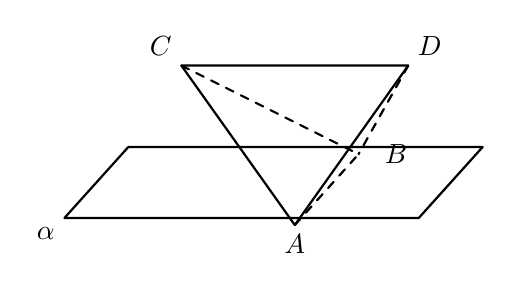
\begin{tikzpicture}[line cap=round,line join=round,x=0.9cm,y=0.9cm]
  \coordinate (C) at (0,2.5);
  \coordinate (D) at (3.2,2.5);
  \coordinate (A) at (1.6,0.25);
  % AB is parallel to the slanted side direction of the alpha plane.
  \coordinate (B) at (2.5,1.25);
  \coordinate (L) at (-0.75,1.35);
  \coordinate (R) at (4.25,1.35);
  \coordinate (Lb) at (-1.65,0.35);
  \coordinate (Rb) at (3.35,0.35);
  \draw[thick] (L)--(R)--(Rb)--(Lb)--cycle;
  \draw[thick] (C)--(D) (C)--(A) (D)--(A);
  \draw[thick,dashed] (C)--(B) (D)--(B) (A)--(B);
  \node[above left] at (C) {$C$};
  \node[above right] at (D) {$D$};
  \node[below] at (A) {$A$};
  \node[right=6pt] at (B) {$B$};
  \node[below left] at (Lb) {$\alpha$};
\end{tikzpicture}
\end{center}
\nopagebreak[4]
\Needspace{4\baselineskip}
\textbf{解析}

令棱 $AB$ 为投影平面内的水平轴。正投影后 $A,B$ 的投影仍相距 $1$，$C,D$ 的投影高度分别是 $u=\frac{\sqrt3}{2}\cos\theta$ 与 $v=\frac{\sqrt3}{6}\cos\theta+\sqrt{\frac23}\sin\theta$（取垂直于 $AB$ 的单位投影方向）。投影凸包面积随方向变化，其极值为 $\frac12\max(|u|,|v|)$（同侧）或 $\frac12(|u|+|v|)$（异侧）。在 $u=v$ 的方向取到最小 $\sqrt2/4$；在 $u,v$ 异号且 $|u-v|=1$ 的方向取到最大 $1/2$。故面积范围为 $[\sqrt2/4,1/2]$。

\gkanswer{答案：$[\sqrt2/4,1/2]$。}

\end{answer}
\begin{answer}
\gksolhead{15}{}

\textbf{题目}：

如图，函数 $y=2\sin(\pi x+\varphi)$，$x\in\mathbb R$（其中 $0\leqslant\varphi\leqslant\dfrac{\pi}{2}$）的图象与 $y$ 轴交于点 $(0,1)$。

（1） 求 $\varphi$ 的值；

（2） 设 $P$ 是图象上的最高点，$M,N$ 是图象与 $x$ 轴的交点，求 $\overrightarrow{PM}$ 与 $\overrightarrow{PN}$ 的夹角。
\nopagebreak[4]
\begin{center}% Source: fixed 2006 Zhejiang science scan, PDF page 1, Q15.
% The plotted phase is schematic but respects the transcribed closed range
% 0 <= phi <= pi/2; M and N are adjacent x-intercepts around peak P.
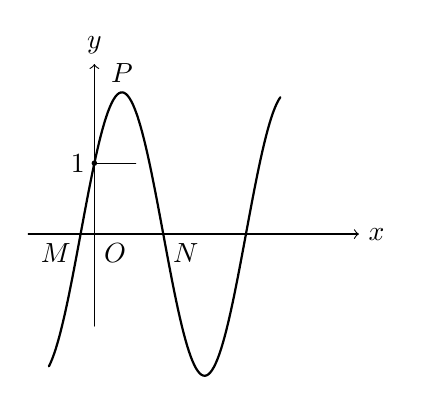
\begin{tikzpicture}[line cap=round,line join=round,x=1.05cm,y=0.9cm]
  \draw[->] (-0.8,0)--(3.2,0) node[right] {$x$};
  \draw[->] (0,-1.3)--(0,2.4) node[above] {$y$};
  \draw[thick] plot[domain=-0.55:2.25,samples=130] (\x,{2*sin(180*\x+30)});
  \draw (0,1)--(0.5,1);
  \node[left] at (0,1) {$1$};
  \fill (0,1) circle (1pt);
  \node[above] at (1/3,2) {$P$};
  \node[below left] at (-1/6,0) {$M$};
  \node[below right] at (5/6,0) {$N$};
  \node[below right] at (0,0) {$O$};
\end{tikzpicture}
\end{center}
\nopagebreak[4]
\Needspace{4\baselineskip}
\textbf{解析}

\gksubpart{(1)}

代入 $(0,1)$ 得 $2\sin\varphi=1$。结合 $0\le\varphi\le\pi/2$，得 $\varphi=\pi/6$。

\gksubpart{(2)}

依源图，最高点 $P$ 两侧相邻零点的横坐标为 $-1/6,5/6$。以 $P=(1/3,2)$ 计算，$\overrightarrow{PM}=(-1/2,-2)$、$\overrightarrow{PN}=(1/2,-2)$。点积为 $15/4$，两向量模长均为 $\sqrt{17}/2$，故夹角余弦为 $15/17$。

\gkanswer{答案（1）：$\varphi=\pi/6$。}

\gkanswer{答案（2）：$\arccos(15/17)$。}

\end{answer}
\begin{answer}
\gksolhead{16}{}

\textbf{题目}：

设 $f(x)=3ax^2+2bx+c$。若 $a+b+c=0$，$f(0)>0$，$f(1)>0$，求证：

（1） $a>0$ 且 $-2<\dfrac ba<-1$；

（2） 方程 $f(x)=0$ 在 $(0,1)$ 内有两个实根。

\Needspace{4\baselineskip}
\textbf{解析}

\gksubpart{(1)}

\Needspace{5\baselineskip}
$c=-a-b$。$f(0)>0$ 给 $a+b<0$，$f(1)>0$ 给 $2a+b>0$，于是 $a>0$ 且 $-2<b/a<-1$。令 $t=-b/a\in(1,2)$，则
\nopagebreak[4]
\[
f(x)=a(3x^2-2tx+t-1).
\]

\gksubpart{(2)}

两根为 $\frac{t\pm\sqrt{t^2-3t+3}}3$，由 $1<t<2$ 可知两根均在 $(0,1)$ 内，故两问结论成立。

\gkanswer{答案（1）：$a>0$ 且 $-2<b/a<-1$。}

\gkanswer{答案（2）：方程 $f(x)=0$ 在 $(0,1)$ 内有两个实根。}

\end{answer}
\begin{answer}
\gksolhead{17}{}

\textbf{题目}：

如图，在四棱锥 $P-ABCD$ 中，底面为直角梯形，$AD\parallel BC$，$\angle BAD=90^\circ$，$PA\perp$ 底面 $ABCD$，且 $PA=AD=AB=2BC$，$M,N$ 分别为 $PC,PB$ 的中点。

（1） 求证：$PB\perp DM$；

（2） 求 $CD$ 与平面 $ADMN$ 所成的角。
\nopagebreak[4]
\begin{center}% Source: fixed 2006 Zhejiang science scan, PDF page 1, Q17.
% Schematic oblique projection; labels and solid/hidden edge relations follow
% the printed figure. M and N lie on PC and PB respectively.
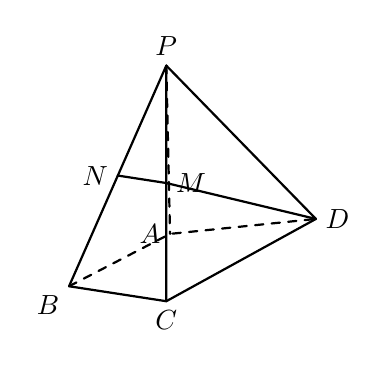
\begin{tikzpicture}[line cap=round,line join=round,x=0.95cm,y=0.95cm]
  \coordinate (P) at (1.55,3.1);
  \coordinate (A) at (1.6,0.85);
  \coordinate (B) at (0.25,0.15);
  \coordinate (C) at (1.55,-0.05);
  \coordinate (D) at (3.55,1.05);
  \coordinate (N) at (0.9,1.63);
  \coordinate (M) at (1.55,1.53);
  \draw[thick] (P)--(B)--(C)--(D)--cycle;
  \draw[thick] (P)--(C) (N)--(M)--(D);
  \draw[thick,dashed] (P)--(A) (B)--(A)--(D);
  \node[above] at (P) {$P$};
  \node[left] at (A) {$A$};
  \node[below left] at (B) {$B$};
  \node[below] at (C) {$C$};
  \node[right] at (D) {$D$};
  \node[left] at (N) {$N$};
  \node[right] at (M) {$M$};
\end{tikzpicture}
\end{center}
\nopagebreak[4]
\Needspace{4\baselineskip}
\textbf{解析}

\gksubpart{(1)}

设 $A=(0,0,0),D=(2,0,0),B=(0,2,0),C=(1,2,0),P=(0,0,2)$。则 $M=(1/2,1,1),N=(0,1,1)$。$\overrightarrow{PB}=(0,2,-2)$、$\overrightarrow{DM}=(-3/2,1,1)$，点积为 $0$，故 $PB\perp DM$。

\gksubpart{(2)}

平面 $ADMN$ 的方程为 $y=z$，法向量可取 $(0,-1,1)$；$\overrightarrow{DC}=(-1,2,0)$，所以线面角 $\theta$ 满足 $\sin\theta=2/\sqrt{10}=\sqrt{2/5}$。

\gkanswer{答案（1）：见解析版}

\gkanswer{答案（2）：$CD$ 与平面 $ADMN$ 所成的角为 $\arcsin\sqrt{2/5}$。}

\end{answer}
\begin{answer}
\gksolhead{18}{}

\textbf{题目}：

甲、乙两袋装有大小相同的红球和白球，甲袋装有 $2$ 个红球、$2$ 个白球，乙袋装有 $2$ 个红球、$n$ 个白球。现从甲、乙两袋中各任取 $2$ 个球。

（1） 若 $n=3$，求取到的 $4$ 个球全是红球的概率；

（2） 若取到的 $4$ 个球中至少有 $2$ 个红球的概率为 $\dfrac34$，求 $n$。

\Needspace{4\baselineskip}
\textbf{解析}

\gksubpart{(1)}

甲取到两红的概率为 $1/6$。当 $n=3$ 时，乙取到两红的概率为 $1/10$。两袋分别抽取，所求概率为 $1/60$。

\gksubpart{(2)}

记乙抽到 $0,1$ 个红球的概率为 $q_0=\frac{n(n-1)}{(n+1)(n+2)}$、$q_1=\frac{4n}{(n+1)(n+2)}$。全体红球少于两个的概率为 $5q_0/6+q_1/6$。令其等于 $1/4$，得 $7n^2-11n-6=0$；正整数解为 $n=2$。

\gkanswer{答案（1）：$1/60$。}

\gkanswer{答案（2）：$n=2$。}

\end{answer}
\begin{answer}
\gksolhead{19}{}

\textbf{题目}：

如图，椭圆 $\dfrac{x^2}{a^2}+\dfrac{y^2}{b^2}=1$（$a>b>0$）与过点 $A(2,0),B(0,1)$ 的直线有且只有一个公共点 $T$，且椭圆的离心率 $e=\dfrac{\sqrt3}{2}$。

（1） 求椭圆方程；

（2） 设 $F_1,F_2$ 分别为椭圆的左、右焦点，$M$ 为线段 $AF_2$ 的中点，求证：$\angle ATM=\angle AF_1T$。
\nopagebreak[4]
\begin{center}% Source: fixed 2006 Zhejiang science scan, PDF page 2, Q19.
% Schematic coordinate drawing; retain ellipse, foci, A/B, tangent point T,
% and the midpoint M of AF_2 with the labelled line segments shown in the scan.
\begin{tikzpicture}[line cap=round,line join=round,x=1.05cm,y=1.05cm]
  \draw[->] (-3.8,0)--(4.2,0) node[right] {$x$};
  \draw[->] (0,-2.25)--(0,2.35) node[above] {$y$};
  % Coordinates follow the stem: a^2=2, b^2=1/2, and c=sqrt(3/2).
  % The tangent AB touches at T=(1,1/2), and M is midpoint of AF_2.
  \draw[thick] (0,0) ellipse (1.41421 and 0.70711);
  \coordinate (A) at (2,0);
  \coordinate (B) at (0,1);
  \coordinate (T) at (1,0.5);
  \coordinate (Fone) at (-1.224745,0);
  \coordinate (Ftwo) at (1.224745,0);
  \coordinate (M) at (1.6123725,0);
  \draw[thick] (B)--(A);
  \draw (Fone)--(T) (T)--(M);
  \fill (Fone) circle (1.3pt) (Ftwo) circle (1.3pt);
  \node[above left] at (B) {$B$};
  \node[above right] at (T) {$T$};
  \node[below] at (A) {$A$};
  \node[below left] at (Fone) {$F_1$};
  \node[below left] at (Ftwo) {$F_2$};
  \node[below right] at (M) {$M$};
  \node[below left] at (0,0) {$O$};
\end{tikzpicture}
\end{center}
\nopagebreak[4]
\Needspace{4\baselineskip}
\textbf{解析}

\gksubpart{(1)}

离心率条件给 $b^2=a^2/4$。直线 $AB$ 为 $x/2+y=1$，与椭圆相切条件给 $a^2/4+b^2=1$，故 $a^2=2,b^2=1/2$，椭圆为 $x^2/2+2y^2=1$，切点 $T=(1,1/2)$。

\gksubpart{(2)}

\Needspace{5\baselineskip}
令 $c=\sqrt{3/2}$。代入 $A,T,M,F_1$ 的坐标可得
\nopagebreak[4]
\[
\tan\angle ATM=\frac{2-c}{2c+1},\qquad
\tan\angle AF_1T=\frac1{2(1+c)}.
\]

恒等式 $2(2-c)(1+c)=2c+1$ 说明两正切相等；两角均为锐角，故角相等。

\gkanswer{答案（1）：$\frac{x^2}{2}+2y^2=1$。}

\gkanswer{答案（2）：见解析版}

\end{answer}
\begin{answer}
\gksolhead{20}{}

\textbf{题目}：

已知函数 $f(x)=x^3+x^2$，数列 $\{x_n\}$（$x_n>0$）的第一项 $x_1=1$，以后各项按如下方式取定：曲线 $y=f(x)$ 在 $(x_{n+1},f(x_{n+1}))$ 处的切线与经过 $(0,0)$ 和 $(x_n,f(x_n))$ 两点的直线平行（如图）。求证：当 $n\in\mathbb N^*$ 时，

（1） $x_n^2+x_n=3x_{n+1}^2+2x_{n+1}$；

（2） $\left(\dfrac12\right)^{n-1}\leqslant x_n\leqslant\left(\dfrac12\right)^{n-2}$。
\nopagebreak[4]
\begin{center}% Source: fixed 2006 Zhejiang science scan, PDF page 2, Q20.
% Schematic graph of y=x^3+x^2 with a secant from O to x_n and a parallel
% tangent at x_{n+1}; vertical guides identify both abscissae.
\begin{tikzpicture}[line cap=round,line join=round,x=1.15cm,y=0.8cm]
  \draw[->] (-0.8,0)--(3.5,0) node[right] {$x$};
  \draw[->] (0,-0.7)--(0,4.9) node[above] {$y$};
  \draw[thick] plot[domain=0:1.62,samples=100] (\x,{\x^3+\x^2});
  % s=0.6 and t=(-1+sqrt(10.12))/2 make f(t)/t=f'(s)=2.28.
  \coordinate (Q) at (0.6,0.576);
  \coordinate (R) at (1.090597372,2.486562008);
  \draw (0,0)--(R);
  \draw (0.18,-0.3816)--(1.02,1.5336);
  \draw[dashed] (0.6,0)--(Q) (1.090597372,0)--(R);
  \node[below left=12pt] at (0,0) {$O$};
  \node[below left=4pt] at (0.6,0) {$x_{n+1}$};
  \node[below right=4pt] at (1.090597372,0) {$x_n$};
\end{tikzpicture}
\end{center}
\nopagebreak[4]
\Needspace{4\baselineskip}
\textbf{解析}

\gksubpart{(1)}

$f'(x)=3x^2+2x$。曲线在 $x_{n+1}$ 处切线的斜率为 $3x_{n+1}^2+2x_{n+1}$；过原点和 $(x_n,f(x_n))$ 的直线斜率为 $f(x_n)/x_n=x_n^2+x_n$。两线平行即得所证。

\gksubpart{(2)}

对固定 $x=x_n>0$，函数 $h(y)=3y^2+2y$ 在正数上严格递增。代入 $y=x/2$ 有 $h(y)=3x^2/4+x<x^2+x$；代入 $y=x$ 有 $h(y)=3x^2+2x>x^2+x$。由（1）得 $x/2<x_{n+1}<x$，归纳并结合 $x_1=1$ 得题中较宽的双边界。

\gkanswer{答案（1）：$x_n^2+x_n=3x_{n+1}^2+2x_{n+1}$。}

\gkanswer{答案（2）：$(1/2)^{n-1}\leqslant x_n\leqslant(1/2)^{n-2}$。}

\end{answer}